\documentclass{article}

\usepackage[preprint]{neurips_2026}

\makeatletter
\renewcommand{\@notice}{}
\makeatother

\usepackage[utf8]{inputenc}
\usepackage[T1]{fontenc}
\usepackage{amsmath}
\usepackage{amssymb}
\usepackage{booktabs}
\usepackage{array}
\usepackage{graphicx}
\usepackage{adjustbox}
\usepackage{caption}
\usepackage{float}
\usepackage{placeins}
\usepackage{xcolor}
\usepackage{hyperref}
\usepackage{url}

\hypersetup{
  colorlinks=true,
  linkcolor=blue,
  citecolor=blue,
  urlcolor=blue
}

\raggedbottom
\setlength{\textfloatsep}{7pt plus 2pt minus 2pt}
\setlength{\intextsep}{7pt plus 2pt minus 2pt}
\setlength{\floatsep}{6pt plus 2pt minus 2pt}
\renewcommand{\topfraction}{0.97}
\renewcommand{\bottomfraction}{0.90}
\renewcommand{\textfraction}{0.03}
\renewcommand{\floatpagefraction}{0.88}
\setcounter{topnumber}{5}
\setcounter{bottomnumber}{4}
\setcounter{totalnumber}{9}
\captionsetup{font=small,skip=3pt}

\newcommand{\pct}{\%\ }

\title{SpherIDiff: A Pilot Experiment on Spherical Weather Inverse Diffusion}

\author{
  Daniyal Hussain Shah
}

\begin{document}

\maketitle

\begin{abstract}
SpherIDiff is a diffusion model for atmospheric data whose spatial operators act on spherical harmonic coefficients. A regional model is obtained from the global model by restricting these operators to the Slepian functions of the region and training a small update. This paper reports a pilot experiment that compares SpherIDiff with the WIND baseline on ERA5 at 5.6 degrees under a fixed budget of 25,000 training steps, and on a regional patch at 1.5 degrees after 5,000 steps of fine-tuning. Three changes made the model practical. Fitting the spherical harmonic transform by least squares raised the usable band limit from 16 to 31 and lowered the error floor of the band-limited target from 0.27 to 0.10. A hierarchy of spectral levels with 16-bit spectral stages reduced the training time from 7.5 times that of the smallest WIND model to between 1.4 and 1.9 times. A local convolution on the sphere gave the largest single gain in accuracy. The best variant reaches a validation error of 0.305 against 0.260 for WIND-S, with fewer parameters (2.96M against 3.01M). Without any training on the patch, it predicts the regional data far better than WIND (0.76 against 1.23), but after fine-tuning it remains behind WIND-S (0.324 against 0.295). A hybrid model that adds convolution and attention blocks matches WIND-S on spatial reconstruction but not on temporal tasks, which suggests that the remaining gap lies in how the model couples space and time. Code and results are available at \url{https://github.com/syeddaniyalg/spheri-diff}.
\end{abstract}

\section{Introduction}

Machine learning models for weather are usually trained on one global grid. WIND~\citep{aich2026wind} is a recent example: a single diffusion model, trained on ERA5, that solves forecasting, downscaling and reconstruction tasks at inference time by posterior sampling. Its layers act on the pixels of a latitude-longitude grid. Such layers have no notion of the sphere, and their weights are tied to the resolution of the grid. A model of this kind cannot be applied directly to a smaller region at a finer resolution.

SpherIDiff takes a different route. Its spatial operators act on spherical harmonic coefficients, which are defined on the sphere itself and do not depend on the grid. For a regional task, the same operators are expressed in the Slepian basis of the region, and only a small part of them is adapted. The idea is that a spectral model should transfer to new regions and resolutions more easily than a grid model, while needing fewer parameters.

This paper reports the pilot experiment that tests this idea at a small scale. It asks two questions. First, can SpherIDiff reach the accuracy of WIND with fewer parameters and a similar training time? Second, does it transfer better to a regional patch at a finer resolution? The experiment follows one model through a sequence of changes, each tested under the same budget, the same data and the same seed. Section~\ref{sec:method} describes the model and the changes, Section~\ref{sec:setup} the experimental setup, Section~\ref{sec:results} the results, and Section~\ref{sec:analysis} what the results show about the remaining gap.

\section{Background}
\label{sec:background}

\paragraph{Diffusion with independent frame noise.}
WIND~\citep{aich2026wind} trains a denoiser on short sequences of atmospheric states. Each frame of a sequence is corrupted with its own noise level, and the network predicts the clean sequence. Because the noise levels are independent, the same network can treat some frames as known context and others as unknown. Forecasting gives the first frame without noise, and reconstruction tasks add the observations through Moment Matching Posterior Sampling (MMPS). The network is not told the noise level of each frame and must infer it from the data. SpherIDiff uses the same training objective and the same inference procedure.

\paragraph{Spherical harmonic operators.}
A field on the sphere that contains only degrees $\ell<L$ is a combination of $K=L^2$ real spherical harmonics. The analysis $T$ maps grid values to these coefficients and the synthesis $S$ maps them back. A spectral layer applies a learned matrix $W$ to the coefficients, which mixes information over the whole sphere in one step. The band limit $L$ sets the finest scale that the layer can represent.

\paragraph{Slepian functions.}
For a region $R$ of the sphere, the Slepian functions are the band-limited functions whose energy is most concentrated in $R$. About $M=\lceil A_R L^2/4\pi\rceil$ of them are well concentrated, where $A_R$ is the area of the region. They are an orthogonal rotation of the spherical harmonics, so a spectral weight $W$ can be restricted to the region as $U_M^\top W U_M$, an $M\times M$ matrix, where $U_M$ holds the first $M$ Slepian functions in harmonic coordinates.

\section{Method}
\label{sec:method}

\subsection{The SpherIDiff block}

The input frames, together with static fields, position and time features, are lifted from 35 channels to a width $d$ at every grid point. Each block then applies three stages, each preceded by a normalisation and added back as a residual:
\begin{equation}
  v \leftarrow v + S\,W\,T\,v, \qquad v \leftarrow v + \text{MLP}(v), \qquad v \leftarrow v + \text{Attention}_t(v).
\end{equation}
The spectral stage mixes over the sphere and is shared by all channels and frames. The channel MLP acts at every grid point. The temporal attention lets the five frames at each grid point attend to each other. A final linear layer maps back to the 25 predicted channels.

\subsection{Choosing the band limit}
\label{sec:bandlimit}

The band limit $L$ sets the finest scale that the model can represent, so the model can only predict a smoothed version of the target. We call the error between the data and its band-limited version the floor, because no model with that band limit can go below it.

The project proposal chose $L$ from the sampling rule of an equiangular grid with $H$ latitudes and $W$ longitudes,
\begin{equation}
  L=\min\bigl(\lfloor (H+1)/2\rfloor,\ \lfloor W/2\rfloor+1\bigr),
\end{equation}
which gives $L=16$ on the $32\times64$ grid. At this limit the floor is 0.274, which is above the validation error of WIND-S (0.260). A model with this band limit therefore cannot reach the baseline, however well it is trained.

We instead chose $L$ empirically, as the band limit with the lowest floor. For each $L$ we transform a field $f$ to coefficients, transform it back, and measure the area-weighted error,
\begin{equation}
  \text{floor}(L)=\bigl\lVert S_L(T_L f)-f\bigr\rVert_a ,
\end{equation}
where the transform $T_L$ is fitted by least squares on the grid points. The floor falls as $L$ grows (Figure~\ref{fig:floor}). The band limit can be raised only while the grid can still tell all harmonics apart, which holds up to $L=H-1=31$ and fails one degree later. Table~\ref{tab:rank} gives both limits on the three grids used by the model. At $L=31$ the floor is 0.101, well below the errors of WIND-S and WIND-M (0.241), so we chose $L=31$.

\begin{table}[htbp]
\centering
\caption{Band limits on the grids of the experiment, from the sampling rule and from least squares.}
\label{tab:rank}
\footnotesize
\begin{tabular}{lrr}
\toprule
Grid & Sampling rule & Least squares \\
\midrule
$32\times64$ & 16 & 31 \\
$16\times32$ & 8 & 15 \\
$8\times16$ & 4 & 7 \\
\bottomrule
\end{tabular}
\end{table}

\subsection{Spectral weights}

The spectral weight $W$ is a dense $K\times K$ matrix, as in the project proposal. At $L=31$ it has 923,521 entries. The first model at $L=31$ used a low-rank form $W=D+PQ^\top$, with $D$ diagonal and rank 32, to stay within the parameter budget; the pooled models of the next section returned to the dense form.

Because $W$ is shared by all channels, every channel receives the same spatial filter. We add one diagonal correction per channel,
\begin{equation}
  W_c = W + \operatorname{diag}\big(\kappa_c(\ell,m)\big),
\end{equation}
which gives each channel $c$ its own weight for every coefficient. The values $\kappa_c$ start at zero, so the model starts as before. A variant with one value per degree, $\kappa_c(\ell)$, was also tested.

\subsection{Pooled levels and 16-bit spectral stages}

The model at $L=31$ runs every block at all 2,048 grid points, which made it 7.5 times slower than WIND-S. The pooled model therefore runs its blocks at three levels, as in a U-Net (Figure~\ref{fig:architecture}). Each level is an equiangular grid with half the height and width of the level above, and its band limit follows the rule of Table~\ref{tab:rank}: $L=31$, 15 and 7. Pooling keeps the degrees below the band limit of the coarser level and synthesises them on the coarser grid. Unpooling synthesises the coarse field on the finer grid, where it is added to the skip connection of that level. The width doubles at each level down, from 64 to 256. The spectral stages and the pooling run in 16-bit precision, which reduced the time per step by 25\pct in a local test without changing the validation error.

\begin{figure}[htbp]
\centering
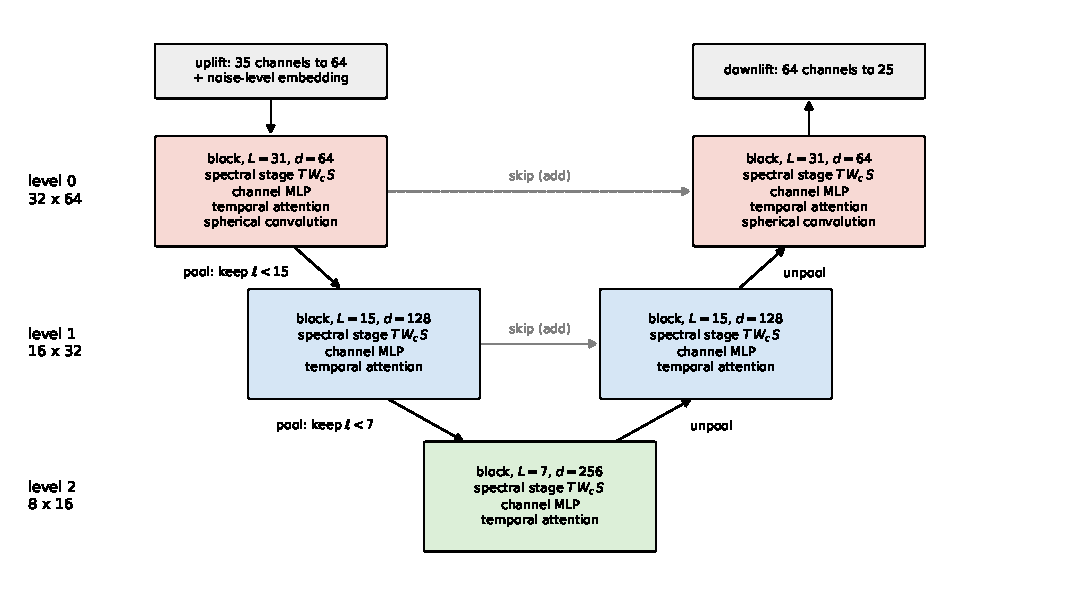
\includegraphics[width=0.92\linewidth]{figures/fig_architecture.pdf}
\caption{The pooled SpherIDiff model with three levels. Pooling and unpooling act on spherical harmonic coefficients. The spherical convolution is present only in the variant of Section~\ref{sec:local}.}
\label{fig:architecture}
\end{figure}

\subsection{Noise-level conditioning}

WIND infers the noise level of each frame from the data. A SpherIDiff block can only do this through a fixed linear spatial operator followed by pointwise layers, which cannot easily compute a nonlinear statistic over a whole frame. We therefore give the network the noise level of each frame through a small embedding that is added after the lift. The noise levels are known in training and in sampling, where the clean context frame has level zero. This is a departure from WIND, and it leaves the training objective unchanged.

\subsection{Local processing}
\label{sec:local}

A spectral stage is global. It is known that global spectral operators learn the large, dominant scales of a field quickly and the weaker, fine scales slowly. We tested two ways to add local processing.

\paragraph{Spherical convolution.}
Following the discrete-continuous convolutions of \citet{ocampo2023disco}, we add a convolution on the sphere at the end of the two blocks of the finest level. The kernel at each point is built from four fixed basis functions of the distance and direction to its neighbours, within a radius of about 5.8 degrees: a central bump, a ring around the point, and the ring weighted by the east-west and north-south direction. They capture a local average, a ring average and the two horizontal gradients. Each output channel is a learned weighted sum of these four local quantities over all input channels. Because the radius is fixed in degrees and each basis function is normalised by its integral over the sphere, the same weights define the same physical operator on the global grid and on the regional patch. The convolution is computed as a sparse matrix product in 16-bit precision. It adds 32,896 parameters and starts at zero.

\paragraph{Hybrid U-ViT.}
The second variant gives the larger share of the model to blocks of the kind used by WIND. At the two finer levels, a residual block with two $3\times3$ convolutions follows the spectral stage; at the coarsest level, a Transformer block attends over all points and all frames. The spectral weight of a level is shared by the blocks on the way down and on the way up, and the noise level conditions the normalisation of every block. About 60\pct of its 2.69M parameters lie in the convolution and Transformer blocks and 37\pct in the spectral weights.

\subsection{Regional fine-tuning}

On the regional patch, each level uses the Slepian functions of the patch at its own band limit. The band limit of the finest level is 120, the least-squares limit of the 1.5-degree grid, and it halves at each coarser level. This gives $M=175$, 44 and 11 Slepian functions for the three levels. The pre-trained weight of each block is restricted to these functions as $G^0=U_M^\top W U_M$ and kept frozen, and a trainable $M\times M$ update $\Delta G$ is added, which starts at zero. With per-channel filters, each channel has its own frozen restricted matrix and $\Delta G$ stays shared. The pointwise layers, the attention and the spherical convolution are fine-tuned as well. Pooling on the patch fits the Slepian functions of the coarser level by least squares, because Slepian bases at different band limits are not nested.

\section{Experimental Setup}
\label{sec:setup}

\paragraph{Data.}
The global data is ERA5 from WeatherBench 2 on an equiangular grid of $32\times64$ points with poles (about 5.6 degrees), every 6 hours. The model predicts the 25 channels listed in Table~\ref{tab:variables}. The training years are 2010 to 2019, validation is 2020 and testing is 2021. Each sample is a window of five frames. The regional patch has $16\times16$ points at 1.5 degrees over Pakistan and northern India (18.0 to 40.5 degrees north, 58.5 to 81.0 degrees east), with training years 2017 to 2019 and the same validation and test years. It is normalised with the statistics of the global training data.

\begin{table}[htbp]
\centering
\caption{The 25 predicted variables.}
\label{tab:variables}
\footnotesize
\begin{tabular}{llr}
\toprule
Variable & Levels & Channels \\
\midrule
Geopotential & 250, 500, 700, 850 hPa & 4 \\
Temperature & 250, 500, 700, 850 hPa & 4 \\
Specific humidity & 250, 500, 700, 850 hPa & 4 \\
Zonal wind ($u$) & 250, 500, 700, 850 hPa & 4 \\
Meridional wind ($v$) & 250, 500, 700, 850 hPa & 4 \\
2 m temperature & surface & 1 \\
Mean sea level pressure & surface & 1 \\
10 m zonal wind ($u$) & surface & 1 \\
10 m meridional wind ($v$) & surface & 1 \\
Total precipitation over 6 hours & surface & 1 \\
\midrule
Total & & 25 \\
\bottomrule
\end{tabular}
\end{table}

\paragraph{Budget and baseline.}
Every model is pre-trained for 25,000 steps and fine-tuned for 5,000 steps with the settings of Table~\ref{tab:config}. The baseline is our re-implementation of WIND at three small sizes, S, M and L, with 3.01M, 7.34M and 12.24M parameters. The WIND models were trained for 45,000 steps; their values at 25,000 steps are interpolated from their evaluations at 24,750 and 27,000 steps.

\paragraph{Measures.}
The validation error is computed every 1,250 steps during pre-training and every 250 steps during fine-tuning, on 32 fixed windows of 2020. Given the first frame without noise, the model generates the next four frames with 3 members and 15 DDIM steps. The error is the area-weighted RMSE of the ensemble mean on standardised fields, averaged over the 25 channels and the four generated frames (nRMSE). The final protocol uses 64 windows of the test year 2021 with 5 members: a forecast of 20 frames, and six reconstruction tasks solved with MMPS, each scored on the unobserved entries. Zero-shot results apply the transferred weights to the patch without any training.

\begin{table}[htbp]
\centering
\caption{Training configuration and hardware.}
\label{tab:config}
\footnotesize
\begin{tabular}{ll}
\toprule
Setting & Value \\
\midrule
Optimiser & AdamW, learning rate $3\times10^{-4}$, no weight decay \\
Schedule & cosine with 5\pct warmup, minimum $10^{-6}$ \\
Batch size / gradient clipping / EMA decay & 16 / 0.8 / 0.999 \\
Steps: pre-training / fine-tuning & 25,000 / 5,000 \\
Precision & 16-bit mixed precision \\
Random seed & 42 \\
Validation & 32 windows of 2020, 3 members, 15 DDIM steps \\
Final protocol & 64 windows of 2021, 5 members, 15 DDIM steps, MMPS \\
Hardware & two NVIDIA T4 GPUs (16 GB) on Kaggle \\
\bottomrule
\end{tabular}
\end{table}

\section{Results}
\label{sec:results}

\subsection{The band-limit floor}

Figure~\ref{fig:floor} shows the floor as a function of the band limit; the global values were discussed in Section~\ref{sec:bandlimit}. The regional patch behaves in the same way: the floor falls from 0.208 at $L'=61$, the quadrature limit of the 1.5-degree grid, to 0.073 at $L'=120$, well below the regional error of WIND-S (0.295).

\begin{figure}[htbp]
\centering
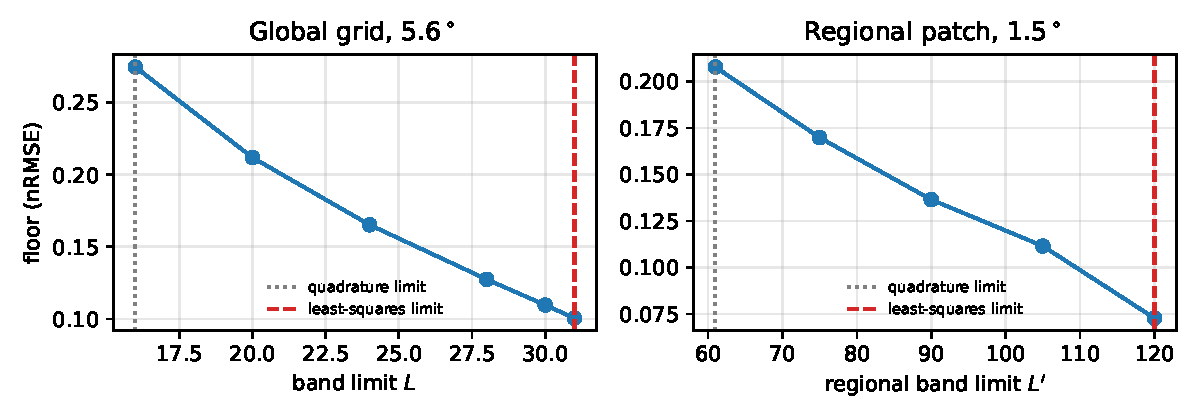
\includegraphics[width=0.9\linewidth]{figures/fig_floor.pdf}
\caption{Floor of the band-limited target, measured on one year of data, for the global grid (left) and the regional patch (right).}
\label{fig:floor}
\end{figure}

\subsection{Accuracy and training time}

Table~\ref{tab:path} follows the model through its main changes, and Figure~\ref{fig:curves} shows the validation curves. Raising the band limit from 16 to 31 lowered the validation error from 0.312 to 0.289, but the model at $L=31$ needed 7.5 times the training time of WIND-S. The pooled model brought the time down to 1.6 times that of WIND-S, at the cost of accuracy (0.340). The per-channel filters and the noise-level conditioning recovered part of this loss (0.323), and the spherical convolution recovered more (0.305), at 1.9 times the training time of WIND-S. Tested one at a time, the per-degree filters lowered the error by 0.016, the noise-level conditioning by 0.010 and an attention over all points at the coarsest level by 0.006.

\begin{table}[htbp]
\centering
\caption{Main models of the experiment. Time is the training time to 25,000 steps on a T4. Global errors are validation errors after 25,000 steps; regional errors are validation errors after 5,000 steps of fine-tuning, and zero-shot errors are the same measure before fine-tuning. The two models at full resolution were fine-tuned with a regional band limit of 61.}
\label{tab:path}
\footnotesize
\begin{adjustbox}{max width=\linewidth}
\begin{tabular}{lrrrrrr}
\toprule
Model & Parameters & Time (h) & s/step & Global nRMSE & Regional nRMSE & Zero-shot nRMSE \\
\midrule
WIND-S & 3,005,369 & \textbf{0.78} & \textbf{0.113} & 0.260 & 0.295 & 1.233 \\
WIND-M & 7,336,121 & 0.91 & 0.131 & \textbf{0.241} & \textbf{0.279} & 1.204 \\
\midrule
SpherIDiff, $L=16$ & 1,601,561 & 3.55 & 0.511 & 0.312 & 0.358 & \textbf{0.515} \\
SpherIDiff, $L=31$ (low rank) & 1,589,277 & 5.88 & 0.849 & 0.289 & 0.358 & 0.815 \\
Pooled & 2,658,238 & 1.24 & 0.179 & 0.340 & 0.340 & 0.828 \\
Pooled + filters + noise level & 2,925,310 & 1.12 & 0.162 & 0.323 & 0.334 & 0.731 \\
Pooled + spherical convolution & 2,958,206 & 1.48 & 0.212 & 0.305 & 0.324 & 0.764 \\
Hybrid U-ViT & 2,685,308 & 0.90 & 0.130 & 0.370 & 0.329 & 0.965 \\
\bottomrule
\end{tabular}
\end{adjustbox}
\end{table}

\begin{figure}[htbp]
\centering
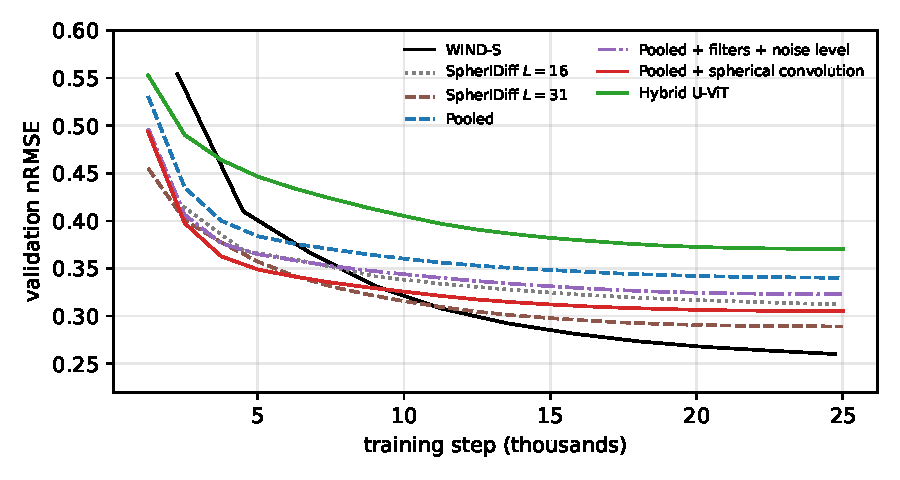
\includegraphics[width=0.78\linewidth]{figures/fig_curves.pdf}
\caption{Validation nRMSE during pre-training.}
\label{fig:curves}
\end{figure}

The SpherIDiff models learn faster than WIND-S at the start. At about 2,500 steps, all of them except the hybrid lie between 0.40 and 0.44, while WIND-S is at 0.55. They then level off, while WIND-S keeps improving and passes them between about 6,500 and 11,000 steps. The hybrid is passed already at about 3,750 steps.

\subsection{Final protocol on the global test year}

Table~\ref{tab:global} reports the final protocol. The WIND models in this table were trained for 45,000 steps, so the comparison favours them. The spherical convolution improves every task over the model without it, most clearly spatial reconstruction (0.548 to 0.506) and spatiotemporal reconstruction (0.437 to 0.398). The hybrid model matches WIND-S on spatial reconstruction (0.454 against 0.457) but is clearly worse on temporal reconstruction (0.398 against 0.224).

\begin{table}[htbp]
\centering
\caption{Final protocol on the global test year 2021. Lower is better. The forecast column gives nRMSE over 20 generated frames; the task columns give nRMSE on the unobserved entries with MMPS. Sp.: spatial, temp.: temporal, s-t: spatiotemporal, rec.: reconstruction, down.: downsampling.}
\label{tab:global}
\footnotesize
\begin{adjustbox}{max width=\linewidth}
\begin{tabular}{lrrrrrrrr}
\toprule
Model & Steps & Forecast & Sp. rec. & Sp. down. & Temp. rec. & Temp. down. & S-t down. & S-t rec. \\
\midrule
WIND-S & 45,000 & 0.422 & 0.457 & 0.342 & 0.224 & 0.217 & 0.383 & 0.332 \\
WIND-M & 45,000 & \textbf{0.400} & \textbf{0.442} & \textbf{0.334} & \textbf{0.199} & \textbf{0.206} & \textbf{0.377} & \textbf{0.319} \\
\midrule
SpherIDiff, $L=31$ (low rank) & 25,000 & 0.480 & 0.572 & 0.456 & 0.255 & 0.267 & 0.479 & 0.443 \\
Pooled + filters + noise level & 25,000 & 0.491 & 0.548 & 0.444 & 0.291 & 0.284 & 0.472 & 0.437 \\
Pooled + spherical convolution & 25,000 & 0.485 & 0.506 & 0.407 & 0.286 & 0.284 & 0.446 & 0.398 \\
Hybrid U-ViT & 25,000 & 0.500 & 0.454 & 0.386 & 0.398 & 0.295 & 0.426 & 0.400 \\
\midrule
Task reference & & & 0.983 & 0.579 & 0.271 & 0.270 & 0.592 & 0.982 \\
\bottomrule
\end{tabular}
\end{adjustbox}
\end{table}

\subsection{Regional transfer and fine-tuning}

Without any training on the patch, every SpherIDiff model predicts the regional data better than WIND (Table~\ref{tab:path}, last column). The best zero-shot result is that of the model at $L=16$ (0.515 against 1.233 for WIND-S); at the higher regional band limit of the pooled models, the zero-shot errors lie between 0.73 and 0.97, because most of the 175 regional Slepian functions contain degrees that the pre-trained weights never saw. After fine-tuning, the spherical convolution gives the best SpherIDiff result (0.324), against 0.295 for WIND-S. Table~\ref{tab:regional} shows the final protocol on the patch. The hybrid model equals WIND-S on spatial reconstruction (0.340) and gives the best SpherIDiff forecast (0.438), but it is again weaker on the temporal tasks. Figure~\ref{fig:gap} summarises the gap to WIND-S along the experiment.

\begin{table}[htbp]
\centering
\caption{Final protocol on the regional test year 2021 after fine-tuning. Columns as in Table~\ref{tab:global}.}
\label{tab:regional}
\footnotesize
\begin{adjustbox}{max width=\linewidth}
\begin{tabular}{lrrrrrrr}
\toprule
Model & Forecast & Sp. rec. & Sp. down. & Temp. rec. & Temp. down. & S-t down. & S-t rec. \\
\midrule
WIND-S & 0.407 & 0.340 & 0.236 & 0.250 & 0.226 & 0.280 & 0.276 \\
WIND-M & \textbf{0.391} & \textbf{0.328} & \textbf{0.230} & \textbf{0.237} & \textbf{0.214} & \textbf{0.272} & \textbf{0.266} \\
\midrule
Pooled + filters + noise level & 0.462 & 0.377 & 0.263 & 0.271 & 0.245 & 0.299 & 0.314 \\
Pooled + spherical convolution & 0.458 & 0.364 & 0.260 & 0.268 & 0.243 & 0.296 & 0.308 \\
Hybrid U-ViT & 0.438 & 0.340 & 0.258 & 0.300 & 0.257 & 0.291 & 0.304 \\
\midrule
Task reference & & 0.956 & 0.319 & 0.271 & 0.225 & 0.354 & 0.953 \\
\bottomrule
\end{tabular}
\end{adjustbox}
\end{table}

\begin{figure}[htbp]
\centering
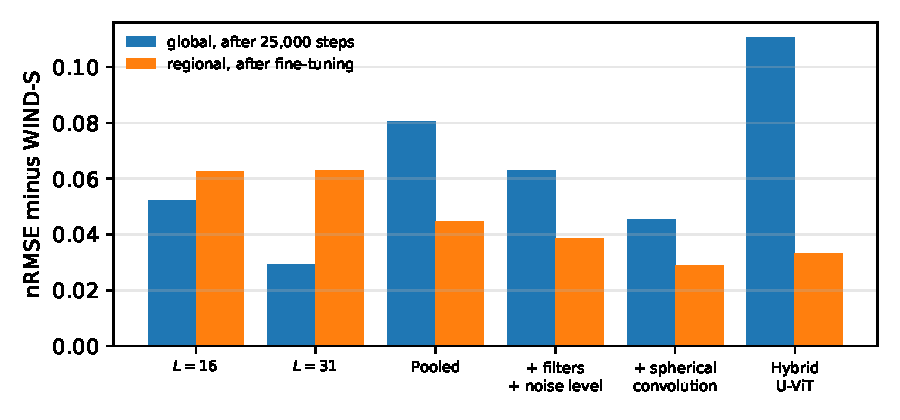
\includegraphics[width=0.78\linewidth]{figures/fig_gap.pdf}
\caption{Validation nRMSE minus that of WIND-S, globally after 25,000 steps and regionally after fine-tuning. The first two models were fine-tuned with a regional band limit of 61, the others with 120.}
\label{fig:gap}
\end{figure}

\section{Analysis}
\label{sec:analysis}

\paragraph{Band-limit floor and remaining error.}
At the least-squares band limits, the floor is 0.10 globally and 0.07 regionally, while the best SpherIDiff errors are 0.305 and 0.324. The remaining error therefore comes from what the network learns within the band, not from what it can represent.

\paragraph{Effect of local processing.}
Of all the changes tested, local processing gave the largest improvement. The SpherIDiff models learn the large scales quickly and then level off (Figure~\ref{fig:curves}), which matches the known behaviour of global spectral operators. Changes to the global filters and the noise-level conditioning each lowered the error by 0.010 to 0.016, and these gains did not carry over to fine-tuning. The spherical convolution, a small local operator with 32,896 parameters, lowered the error by 0.018 and improved the regional result as well. It also kept most of the zero-shot advantage over WIND, because its kernel is defined in degrees.

\paragraph{Coupling of space and time.}
The two local variants differ mainly in how they treat time. The hybrid model has local convolutions and an attention over all points and frames, and it matches WIND-S on spatial reconstruction globally and regionally. Its frames interact only in one Transformer block at the coarsest level, and it is clearly weaker on temporal reconstruction and on the validation forecast, which depends on the evolution between frames. The pooled models keep a temporal attention at every level and do better on these tasks. This contrast suggests that the remaining gap to WIND lies in how the model couples space and time, rather than in either alone.

\paragraph{Changes without benefit.}
Three changes did not improve the model. A low-rank spectral weight matched the dense weight in validation but gave much worse long forecasts in the pooled model (0.765 against 0.555 over 20 frames). A fourth pooling level made the model faster but less accurate (0.369 against 0.340). An attention over all points at the coarsest level lowered the error by only 0.006.

\section{Reproducibility}

All runs use the seed 42 and the configuration of Table~\ref{tab:config}. Each Kaggle notebook in the repository runs one experiment from pre-training to the final regional evaluation, and each model variant is selected by its configuration file. The figures of this paper are produced by \texttt{paper/make\_figures.py} from the result files in the repository.

\section{Limitations}

Every result comes from one seed. Two runs of the same model differed by about 0.008 after 1,000 steps; the difference after 25,000 steps was not measured, so small differences between variants are not conclusive. The WIND references were trained for 45,000 steps, so their 25,000-step values are interpolated and the final tables favour them. The experiment uses one coarse resolution and one region. Training times were measured in different Kaggle sessions and vary by a few percent between sessions. The noise-level conditioning departs from the framework of WIND, although its measured effect was small. Finally, the least-squares rule was checked on the grids of Table~\ref{tab:rank}; for the 1.5-degree grid it was checked only through the regional fit, which gave a unique solution with 175 functions on 256 points.

\section{Conclusion}

The pilot experiment shows that a spherical spectral diffusion model can be made practical at a small scale. Least squares removed most of the band-limit floor, and pooled levels with 16-bit spectral stages brought the training time close to that of WIND-S. With a local convolution on the sphere, SpherIDiff reaches a validation error of 0.305 against 0.260 for WIND-S, with fewer parameters, and it transfers to a new region and resolution far better before fine-tuning. It does not yet match WIND-S after training or after fine-tuning. The results point to the coupling of space and time as the next part of the model to improve.

\begin{thebibliography}{2}

\bibitem[Aich et~al.(2026)]{aich2026wind}
Michael Aich, Andreas F{\"u}rst, Florian Sestak, Carlos Ruiz-Gonzalez, Niklas Boers, and Johannes Brandstetter.
\newblock WIND: Weather inverse diffusion for zero-shot atmospheric modeling.
\newblock \emph{arXiv preprint arXiv:2602.03924}, 2026.

\bibitem[Ocampo et~al.(2023)]{ocampo2023disco}
Jeremy Ocampo, Matthew Price, and Jason McEwen.
\newblock Scalable and equivariant spherical CNNs by discrete-continuous (DISCO) convolutions.
\newblock In \emph{International Conference on Learning Representations}, 2023.

\end{thebibliography}

\end{document}
